The frontier at threshold $50\%$ has a direct seat interpretation. With two-party shares a district is Democratic-majority exactly when it is not Republican-majority, so under a regime $\rho$ the number of Democratic-majority districts of any plan lies between $k-F^{R}_\rho(0)$ and $F^{D}_\rho(0)$, and both ends are attained by some plan (Proposition~\ref{prop:mono}(4) gives the Republican side from the same code). Certified bounds on $F^D$ and $F^R$ therefore give a certified \emph{seat range} for each state; Table~\ref{tab:enacted} and Figure~\ref{fig:seatrange} report it next to the delegation of the enacted 118th-Congress plan and the seat count that would be proportional to the statewide vote. All counts use the two-party 2020 presidential vote in each district; they are descriptions of vote geography, not predictions of congressional results. (A district with an exactly tied two-party vote would count for both parties at threshold 50\%, so the range is exact up to such ties.)

\begin{table}[!tbp]
\centering\footnotesize
\caption{Seat range under $\rho_s$ at threshold 50\% and the enacted plans (2022 elections; each rendered at precinct resolution, Section~\ref{sec:data}). Columns give numbers of Democratic-majority districts: ``enacted'' for the enacted plan; ``verified'' the smallest and largest count attained by independently verified plans of $\rho_s$; ``limits'' what the infeasibility proofs leave possible. Splits are $\sum_K(d_K-1)$ of the rendered plan with the budget $s$ of $\rho_s$ in parentheses; ``in $\rho_s$'' says whether the rendered plan satisfies $\rho_s$ (population within $\pm1\%$, connected, at most $k-1$ splits).}\label{tab:enacted}
\adjustbox{max width=\linewidth}{\begin{tabular}{lrrcccrrc}
\toprule
State & $k$ & D share & enacted & verified & limits & splits ($s$) & max.\ dev. & in $\rho_s$ \\
\midrule
New Hampshire & 2 & 53.7\% & 2 & 2 & 2 & 5 (1) & 0.00\% & no \\
Maine & 2 & 54.7\% & 1 & 1--2 & 1--2 & 1 (1) & 0.00\% & yes \\
Rhode Island & 2 & 60.6\% & 2 & 2 & 2 & 1 (1) & 0.19\% & yes \\
Idaho & 2 & 34.1\% & 0 & 0 & 0 & 1 (1) & 0.02\% & yes \\
Montana & 2 & 41.6\% & 0 & 0--1 & 0--1 & 1 (1) & 0.07\% & no \\
West Virginia & 2 & 30.2\% & 0 & 0 & 0 & 0 (1) & 0.09\% & yes \\
Nebraska & 3 & 40.2\% & 1 & 0--1 & 0--2 & 2 (2) & 0.37\% & yes \\
New Mexico & 3 & 55.5\% & 3 & 1--3 & 1--3 & 10 (2) & 0.64\% & no \\
Arkansas & 4 & 35.8\% & 0 & 0--1 & 0--2 & 3 (3) & 0.05\% & yes \\
Iowa & 4 & 45.8\% & 0 & 0--3 & 0--3 & 0 (3) & 0.01\% & yes \\
Kansas & 4 & 42.5\% & 1 & 0--2 & 0--3 & 4 (3) & 0.05\% & no \\
Mississippi & 4 & 41.6\% & 1 & 0--2 & 0--3 & 4 (3) & 0.12\% & no \\
Nevada & 4 & 51.2\% & 3 & 1--3 & 1--4 & 3 (3) & 0.36\% & yes \\
Utah & 4 & 39.3\% & 0 & 0--2 & 0--2 & 7 (3) & 0.76\% & no \\
Connecticut & 5 & 60.2\% & 5 & 4--5 & 4--5 & 10 (4) & 0.77\% & no \\
Oklahoma & 5 & 33.1\% & 0 & 0--1 & 0--2 & 7 (4) & 0.21\% & no \\
\bottomrule
\end{tabular}
}
\end{table}

\begin{figure}[!tbp]
\centering
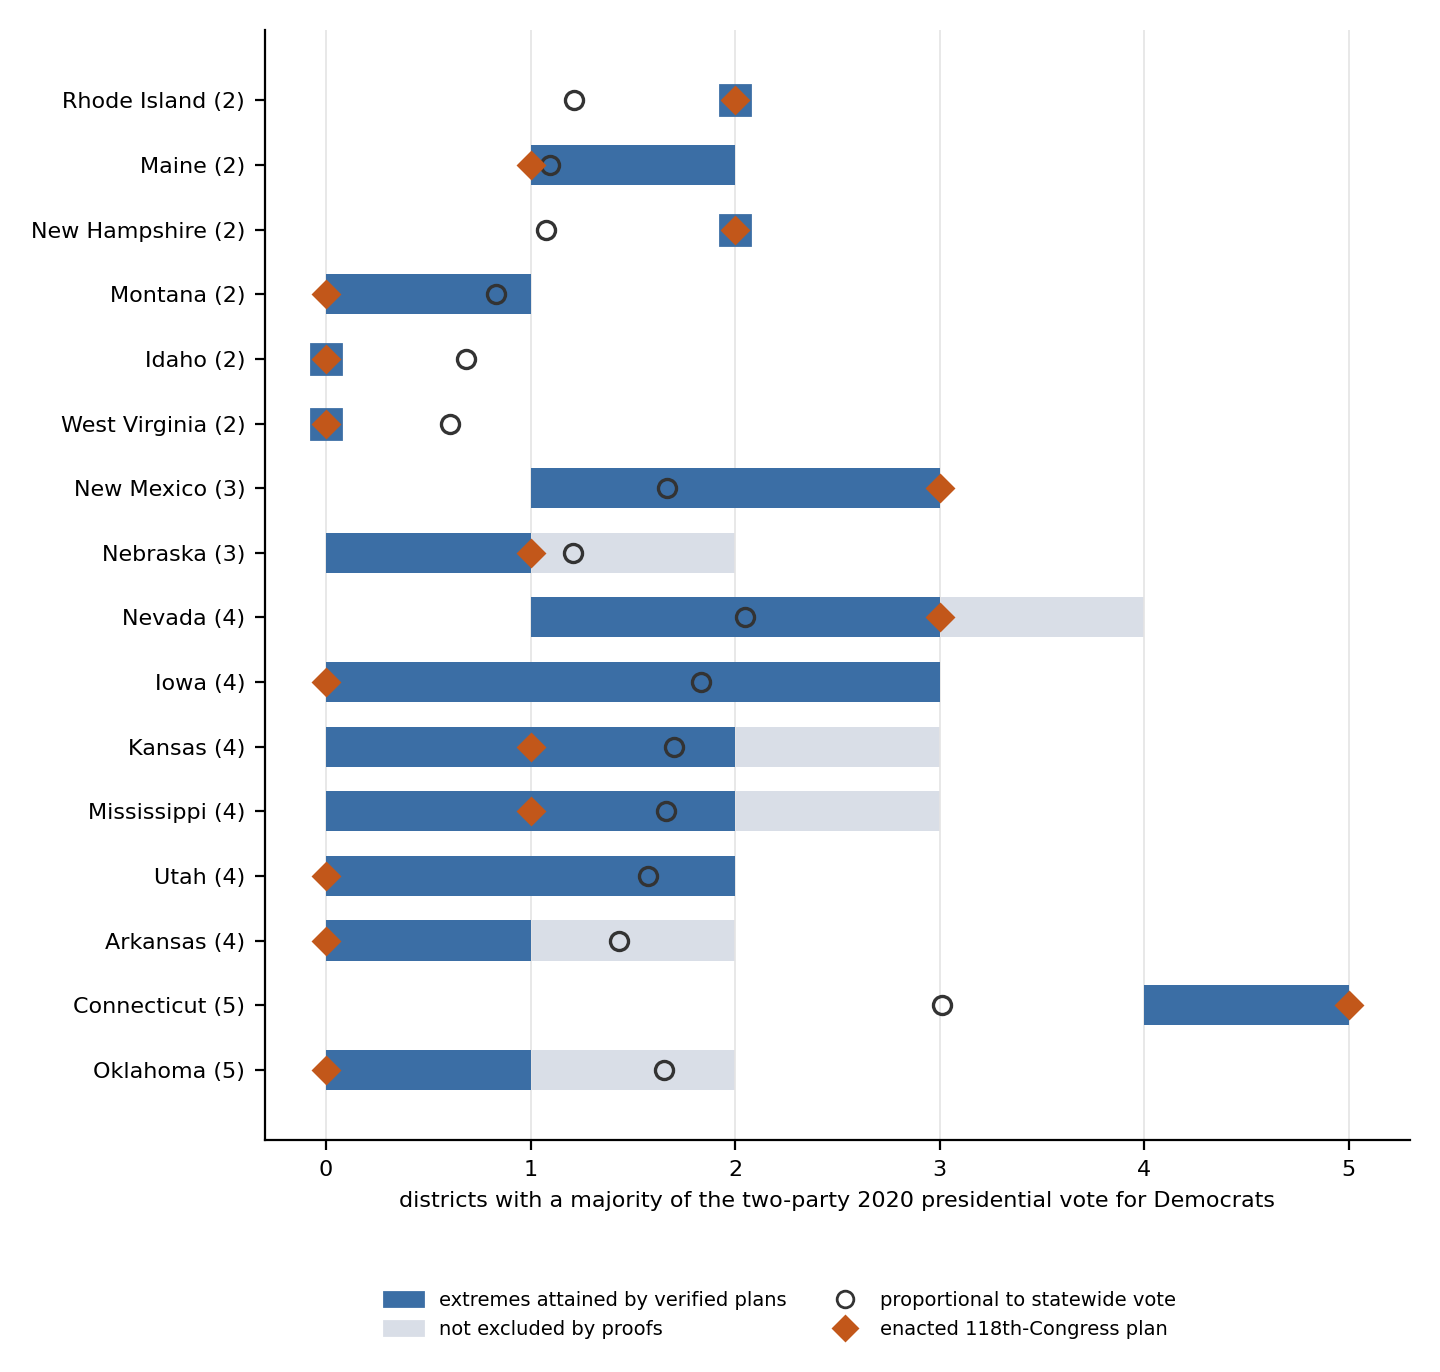
\includegraphics[width=0.86\linewidth,height=0.6\textheight,keepaspectratio]{figs/seatrange.png}
\caption{Certified range of the number of Democratic-majority districts under $\rho_s$ (threshold 50\% of the two-party 2020 presidential vote), the delegation of the enacted plan, and proportionality. Both extremes of the dark bar are attained by verified plans; light grey marks counts that the proofs do not exclude. Intermediate counts are not claimed to be attained.}\label{fig:seatrange}
\end{figure}

\paragraph{Where line drawing decides and where geography does.}
In four of the 16 states (New Hampshire and Rhode Island for Democrats, Idaho and West Virginia for Republicans) the delegation is the same for every plan of $\rho_s$: the two ends of the certified range coincide (Table~\ref{tab:enacted}). In the other twelve, verified plans attain a spread of one to three seats, and the proofs leave at most one further seat open in six of them; summed over the 52 seats of the 16 states, verified plans move the Democratic count between $11$ and $30$ and the proofs exclude anything below $11$ or above $36$ (the separability of Proposition~\ref{prop:sep} makes such sums valid for the union of states). Verified plans give Republicans a majority of the delegation in twelve of the 16 states and Democrats in seven; Iowa, Nevada and New Mexico are in both lists, and in New Hampshire, Rhode Island, Maine and Connecticut only Democrats can (in Maine Republicans can hold at most one of the two seats). Both parties are run through identical code, so which side has this capacity is a property of each state's vote geography and the regime. The Democratic delegations of the enacted plans total 19 of 52 seats (proportionality to the statewide votes would give 23.3), inside the verified range of 11 to 30.

\paragraph{The enacted plans in context.}
The rendered enacted plans are outside the regime in eight states, mainly because they split more counties than $k-1$ (Table~\ref{tab:enacted}; Montana's rendering has one detached precinct of 530 residents), and were drawn under criteria our model does not include, so their position relative to the range is a description and no evidence about intent. With that caveat, three observations are certified. First, in each of the 71 (state, party, $q$) combinations for which a verified plan has a $q$-th district above 50\%, the $q$-th best district of the enacted plan is below the certified lower end of $\sigma^*(q)$: by a median of 5.9 points of district share (5.4 points for the 28 single-best-district cases; smallest gap 0.2, largest 23.4; Figure~\ref{fig:scatter}, diamonds). No enacted plan exhausts what boundaries could do for either party at any rank, although a single plan cannot exhaust all ranks at once. Second, the delegation of the enacted plan lies at an end of the verified seat range in ten of the twelve states in which the range is not a single value, and in the interior in two (Kansas and Mississippi, each with one Democratic seat in a verified range of $0$--$2$); the end is the Republican end (fewest Democratic seats) in six of the ten and the Democratic end in four. Third, the enacted plans supply an independent test of the bounds: the eight of them that satisfy $\rho_s$ are ordinary plans of the regime, shaped by others (the test concerns the rendered plans, which are verified plans of $\rho_s$ whatever their fidelity to the enacted maps), and none of their 46 (party, $q$) margins reaches the proven upper end of the corresponding bracket, while none exceeds a lower end, so no plan in the public record improves our lower bounds in these states.
